\chapter{Technische Umsetzung}

Die technische Umsetzung der durchgeführten Analyse ist von der
Pipeline Architektur inspiriert. Die geschriebenen Skripts profitieren
von der isolierten Natur der Aufgabe und wenden wo immer möglich
funktionale Prinzipien wie Immutability, Higher Order- und Pure Functions
an.

Die untenstehende Abbildung \ref{flowchart-aggregation} zeigt den
grundsätzlichen Ablauf der Analyse der Daten. Dabei implementiert
die Software sowohl Aspekte des Batch- wie auch des Stream Processings.
Einerseits läuft die Auswertung von Anfang bis zum Schluss auf dem gesamten
Datensatz durch, andererseits nutzt sie einen MongoDB Cursor, der die
Artikel aus der DB Stück für Stück herunterlädt (streamt). Dieser Cursor ermöglicht
es dem Programm, bereits heruntergeladene Artikel zu analysieren und nach
Abschluss wieder aus dem Speicher zu löschen, um Ressourcen zu schonen.
Des Weiteren verwendet das Skript einen Processor Pool, der die gleichmässige
Verteilung der Last auf alle CPU Kerne garantiert und damit die zur Verfügung
stehenden Ressourcen ganz ausnutzt.

\begin{figure}[H]
	\begin{center}
        \centering
		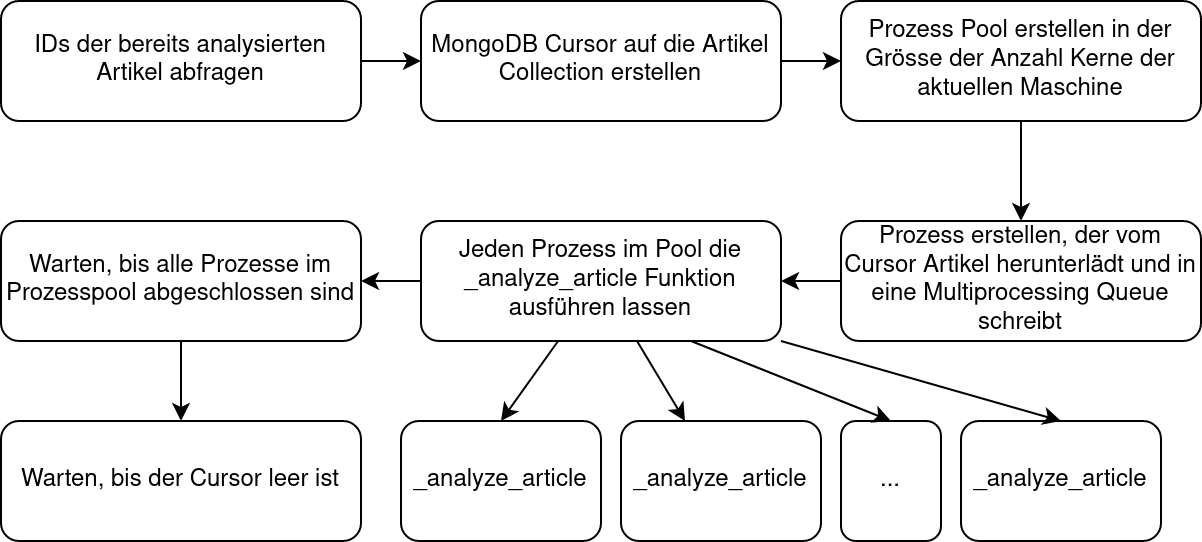
\includegraphics[width=1\linewidth]{./images/aggregate.png}
	\end{center}
	\caption{Ablaufdiagramm der Auswertung}
	\label{flowchart-aggregation}
\end{figure}

Die Abbildung \ref{aggregation-function} zeigt den Python Code,
der über den Prozessor Pool auf die einzelnen CPU Kerne verteilt wird.
Diese Funktion konsumiert Artikel aus der \enquote{articles\_queue},
einer Multiprocessing-sicheren Datenstruktur, die nach und nach vom
MongoDB Cursor mit Artikeln aus der DB gefüllt wird.
Die Funktion läuft so lange, bis sie für mindestens zehn Minuten
keine neuen Artikel in der Queue mehr findet. Der Grund für dieses eher hohe
Timeout sind mögliche Netzwerkprobleme oder andere unvorhergesehene
Unterbrüche. Bei Verarbeitung solch grosser Datenmengen fallen die
zusätzlichen 10 Minuten nicht ins Gewicht und sind betreffend
Performanz zu vernachlässigen.
Nach dem Erhalt eines neuen Artikels bestimmt der Algorithmus,
ob der aktuelle Artikel bereits analysiert wurde.
Falls ja, verwirft er ihn wieder und holt sich einen neuen.
Danach beginnt die effektive Analyse. Einzelne Funktionen daraus sind
in den nachfolgenden Kapiteln näher beschrieben.
Als nächstes bestimmt die Funktion das Geschlecht des Autors, danach durchsucht
sie den Text nach Personen und Zitaten. Zum Schluss weist sie
die gefundenen Personen den gefundenen Zitaten zu und speichert das
Resultat in der Datenbank.
Wenn die Abfrage der Queue in ein Timeout läuft (zehn Minuten), dann
wirf die Funktion eine \enquote{Empty} Exception, die vom \enquote{except}
Block abgefangen wird und dazu führt, dass die Funktion und damit der
Prozess beendet wird.

\begin{figure}[H]
    \begin{lstlisting}[language=Python]
def _analyze_article(processor_nr: int) -> None:
    log.info("Starting processor %d", processor_nr)
    while True:
        try:
            article_dict = articles_queue.get(
                timeout=600
            )  # 10min, in case of network issues

            if article_dict["_id"] in analyzed_articles:
                continue

            builder = ArticleBuilder()
            article = builder.from_db_result(article_dict).build()

            genderized_author = get_genderized_person(
                get_person_from_string(article["author"])
            )

            article_text = article["text"]
            people = get_people_from_string(article_text)
            genderized_people = map(get_genderized_person, people)

            citations = get_syntactic_quotes(article_text)
            citations_with_person = assign_people_to_citations(
                genderized_people, citations
            )

            analyzed_article = get_analyzed_article(
                article, genderized_author, citations_with_person
            )
            insert_analyzed_article(analyzed_article)

        except Empty:
            log.info("Queue is empty! Terminating processor %d!", processor_nr)
            return
    \end{lstlisting}
    \caption{Funktion: \_analyze\_article()}
    \label{aggregation-function}
\end{figure}

\newpage
\section{Datensammlung bereinigen}

Die Vorarbeit hat eine Datensammlung von etwa 370'000 Nachrichtenartikeln ergeben, die jeweils über eine eindeutige URL verfügen. 
Wir haben durch die Verwendung von Unique Constraints sichergestellt, dass jede URL einzigartig ist. 
Allerdings vermuteten wir, dass die Datensammlung Duplikate von Texten enthält, die unter verschiedenen URLs veröffentlicht wurden. 
Dies könnte durch Weiterleitungen auf andere Seiten oder veränderte URLs verursacht worden sein. 
Um eine genaue Aussage über den Gender Gap in diesen Nachrichtenportalen machen zu können, mussten wir alle Duplikate pro Nachrichtenportal eliminieren. 

Nach einigen Testversuchen mit 1000 Artikeln entschieden wir uns dafür, die \gl{cosine-similarity} zu verwenden, um Artikeltexte untereinander zu vergleichen. 
Dieser Vergleich war bei den Tests performanter als die \gl{levenshtein-similarity}, die ebenfalls zur Auswahl stand. 
Der Rechenaufwand für den Vergleich zweier Zeichenketten der Länge m bzw. n ist bei der \gl{levenshtein-similarity} 
\(O(m*n)\), während er bei der \gl{cosine-similarity} nur \(O(m+n)\) beträgt
\footnote{https://pypi.org/project/strsimpy/}.

Die \gl{cosine-similarity} ist eine Metrik zur Messung der Ähnlichkeit zwischen zwei Vektoren.
Sie definiert die Ähnlichkeit zwischen zwei Vektoren als den Kosinus des Winkels zwischen ihnen.
In unserem Fall sind die Vektoren die Artikeltexte repräsentiert im Vector Space Modell. 
Um die Ähnlichkeit zwischen einem Vektor und einer Menge von anderen Vektoren zu berechnen, erstellen wir eine Ähnlichkeitsmatrix. 
Wenn der Kosinus 1 ist, sind die Texte gleich. 
Als Schwellwert für die Ähnlichkeit haben wir 0.9 festgelegt, da dieser bei unseren Tests am besten funktionierte. 
Wenn wir einen höheren Schwellwert genommen hätten, hätten wir nicht alle Duplikate gefunden und bei einem zu niedrigen Schwellwert
hätten wir zu viele Texte als Duplikate interpretiert, die gar keine sind. 

Da jeder Artikeltext mit jedem anderen verglichen werden muss, hätte der Algorithmus eine Matrix in der Grösse 
von 371'653 x 371'653 erstellen müssen und 42,9 GB Arbeitsspeicher benötigt. 
Das war für unsere Arbeitsmaschinen zu viel. 
Daher haben wir das \enquote{divide and conquer} Verfahren angewendet und aus einem grossen Problem kleine Teilprobleme gemacht. 
Für jeden Artikel, den wir verglichen haben, haben wir eine neue Matrix erstellt, sodass sie nur noch 1x371'653 gross war und dann nacheinander 371'653 Mal verglichen wurde. 
Wir gingen damit einen Tradeoff ein, der die Ausführungszeit verlängerte, die der Algorithmus benötigte. Das erstellte Skript benötigte zwei Tage um alle Duplikate zu finden.

Auf diese weise konnten wir alle Duplikate und nahezu-Duplikate aus der Datenbank entfernen.
Die Abbildung \ref{duplicates} gibt einen Überblick über die entfernten Artikel pro Nachrichtenportal.

\begin{figure}[H]
	\begin{center}
        \centering
		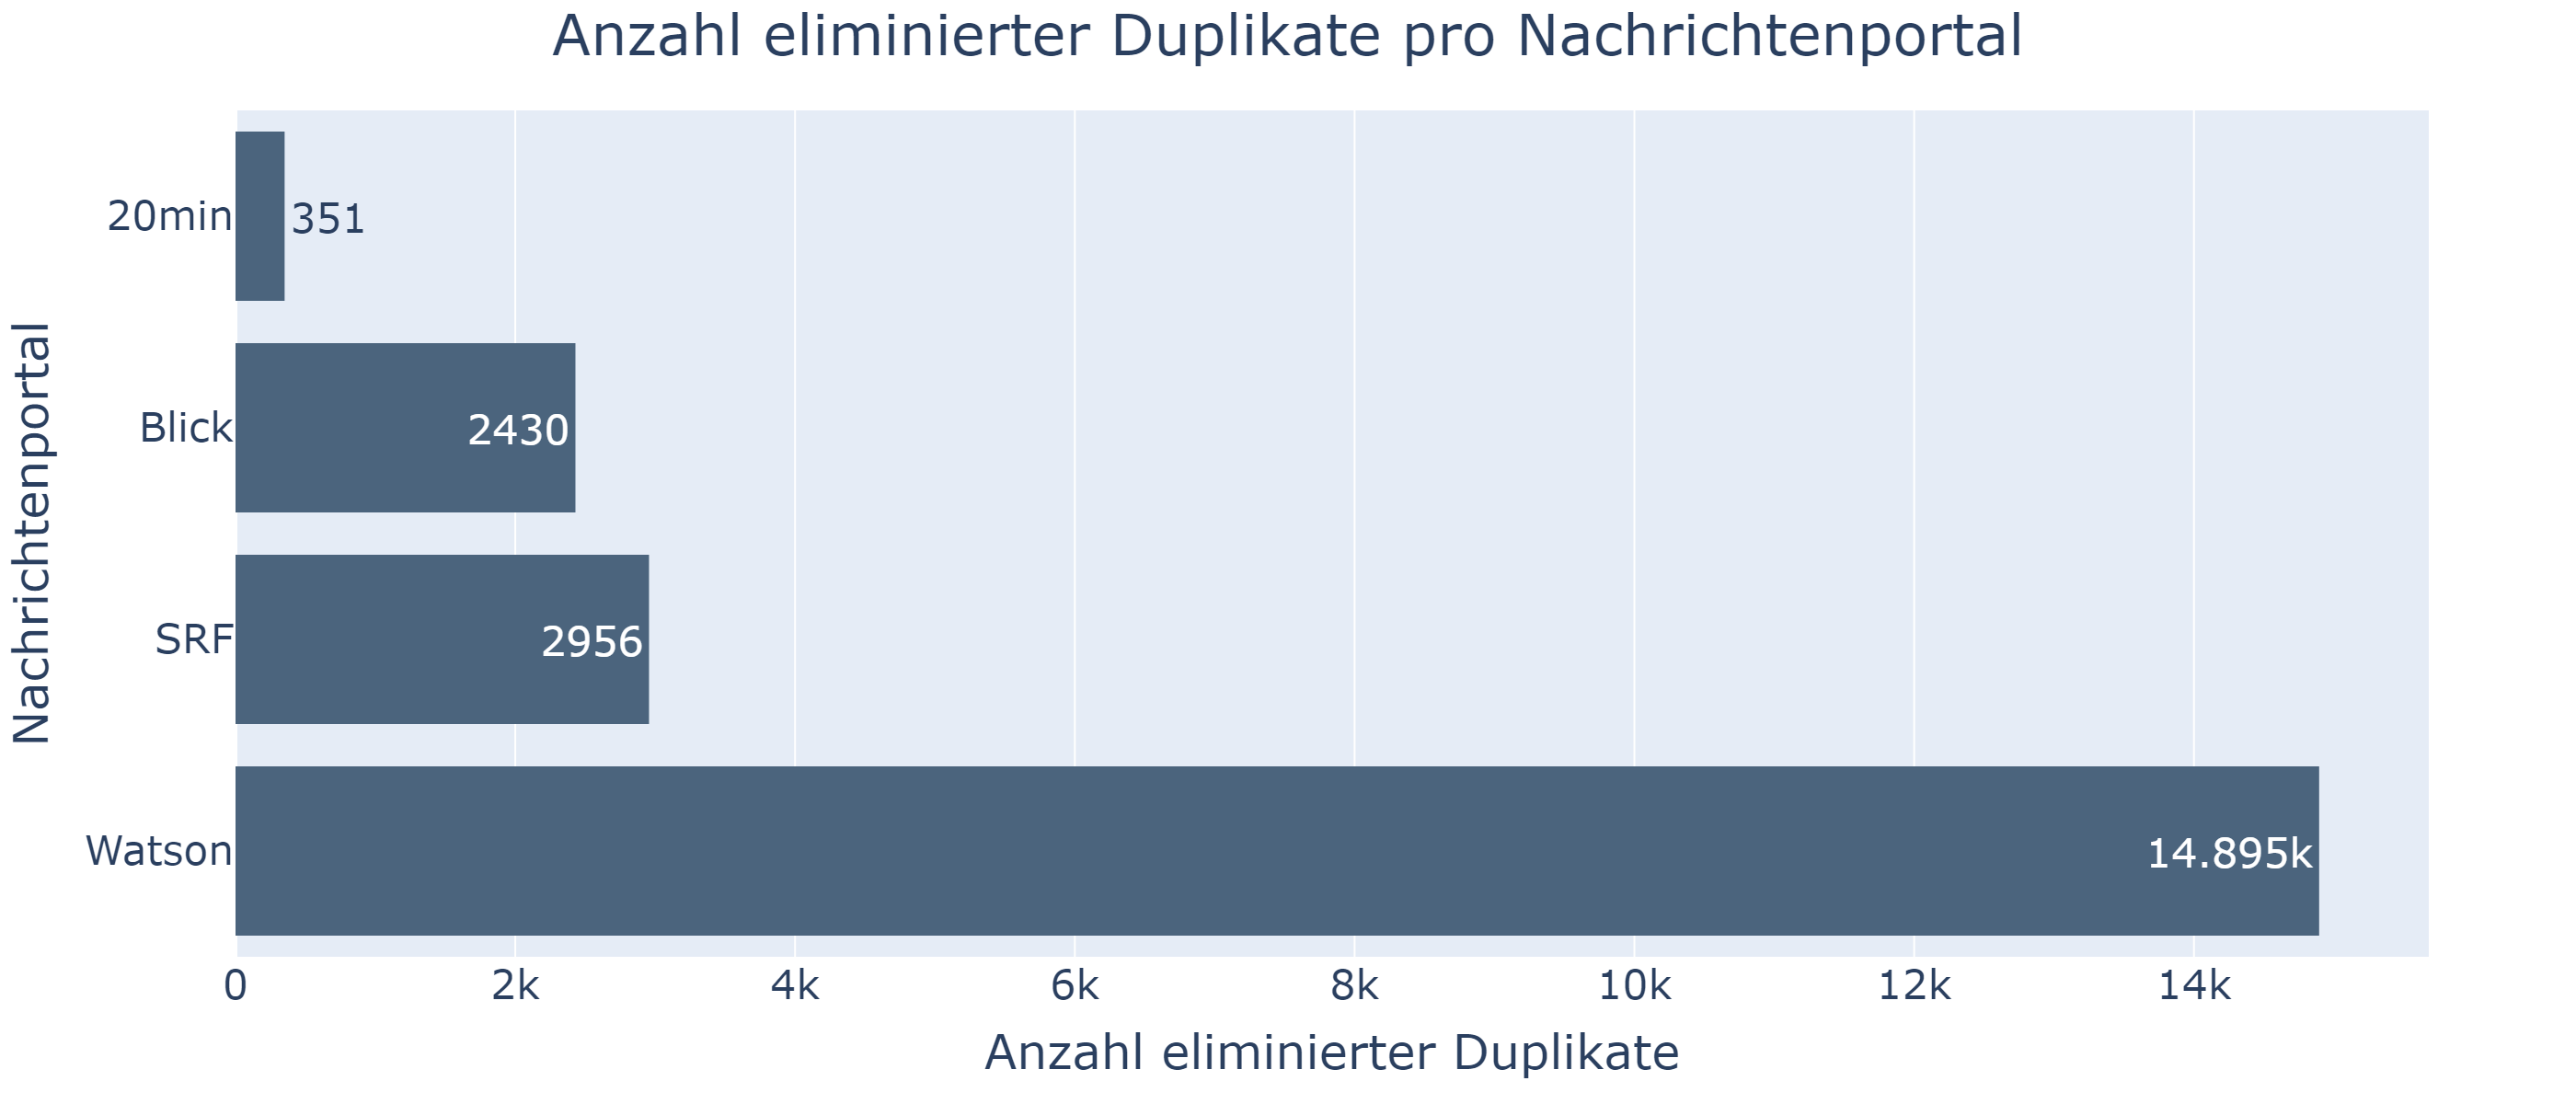
\includegraphics[width=1\linewidth]{./images/duplicates_count.png}
		\caption{Anzahl eliminierter Duplikate pro Nachrichtenportal}
		\label{duplicates}
	\end{center}
\end{figure}

\newpage
\section{Datenbank}\label{db-design}
Wir haben im Vorprojekt von der BFH eine virtuelle Maschine gemietet, auf die wir über \ashort{ssh} zugreifen können.
Auf dieser haben wir eine MongoDB installiert, um dort die Artikel zu speichern.
Die \gl{collection} \enquote{analyzed\_articles} enthält die analysierten Artikel.
Diese enthalten die gefundenen Zitate mit Personen und deren Geschlecht.
Die Struktur der Einträge ist in Abbildung \ref{structure-analyzed-articles} ersichtlich.
Darunter in der Abbildung \ref{analyzed-article} folgt ein Eintrag der DB als Beispiel.

% \newlist{myEnumerate}{itemize}{3}
% \setlist[myEnumerate]{nosep,label=\protect\mpbullet}
% \setlistdepth{6}
\begin{figure}[H]
\textbf{analyze\_articles}
\begin{itemize}
    \item \textbf{title:} Titel des Artikels
    \item \textbf{lead:} Lead Text des Artikels
    \item \textbf{url:} \ashort{url} zum Artikel, eindeutiger Schlüssel
    \item \textbf{author:} Autor:in des Artikels
    \item \textbf{source:} Das Nachrichtenportal
    \item \textbf{published:} Timestamp der Veröffentlichung
    \item \textbf{updated:} Timestamp der letzten Aktualisierung
    \item \textbf{text:} Text des Artikels
    \item \textbf{quotes:} Zitate in Form von Liste
    \begin{itemize}
        \item \textbf{designation:} Person von Zitat
        \item \textbf{gender:} Geschlecht der Person
        \item \textbf{quotation verb:} Verb welches zum Zitat einleitet
        \item \textbf{quote:} Zitat Text
        \item \textbf{start of quote in text:} Start Position von Zitat im Text
    \end{itemize}
\end{itemize}
\caption{Struktur eines Eintrags in der MongoDB Collection \enquote{analyzed\_articles}}
\label{structure-analyzed-articles}
\end{figure}

\newpage

\begin{figure}[H]
	\begin{lstlisting}
{
    "_id": "794aceeeea0911eda58075d660e6a249",
    "article": {
        "_id": "cf49cff695fa11ed8a280242ac110002",
        "title": "Nimm dich nicht zu wichtig!",
        "lead": "Bescheidenheit ist eine Zier, doch weiter kommt man ohne ihr, besagt ein Sprichwort. Doch zahlt sich Bescheidenheit wirklich weniger aus als Selbstdarstellung? Eine Bestandesaufnahme.",
        "author": {
            "designation": "Raphael Zehnder",
            "gender": "male"
        },
        "source": "srf",
        "url": "www.srf.ch/kultur/gesellschaft-religion/wochenende-gesellschaft/
        bonus-bescheidenheit-nimm-dich-nicht-zu-wichtig",
        "published": 1577005620,
        "updated": 1577005620,
        "text": "Egozentrische Pfauen tummeln sich allenthalben: Wirtschaftskapitäne blasen sich auf, Politikerinnen und Politiker lobpreisen ..."
    },
    "quotes": [
        {
            "subject": {
                "designation": "Walter Slezak",
                "gender": "male"
            },
            "quotation_verb": "brachte",
            "quote": "Wir kaufen Dinge, die wir nicht brauchen, um Menschen zu beeindrucken, die wir nicht mögen",
            "start_of_quote_in_text": 555
        }
    ]
}
        
	\end{lstlisting}
	\caption{\enquote{analyzed\_articles} \gl{collection} Eintrag Beispiel}
	\label{analyzed-article}
\end{figure}

\newpage
\section{Personen extrahieren}\label{people-extraction}

% 1. NER Entitäten mit Personen Tag aus Text lesen
% 2. Mit Coreference resolution Personen Cluster bekommen
% 3. NER Coreference und Coref-Res Entitäten verbinden um eindeutige Personen zu bekommen mithilfe der Schnittmenge der Wörter
% Dabei wird aus den Coreference Einträge neben Vornamen und Nachnamen der Person auch noch Pronomen und Artikel herausgelesen mit POS und der Person zugewiesen.
% diese sind dann zusätzlich zum Vornamen hilfreich für das Geschlecht der Person zu bestimmen.

Das Extrahieren von Personen aus einem Text umfasst mehrere Schritte.
Zunächst werden die Entitäten mit dem Tag \enquote{Person} mithilfe von \gl{ner} aus dem Text herausgelesen.
Als Nächstes wird \gl{cr} verwendet, um Personencluster zu bilden. 
Dies bedeutet, dass der Text auf Referenzen zu Personen überprüft wird, z.B. wenn eine Person im Text als \enquote{sie} oder \enquote{er} bezeichnet wird. 
\gl{cr} hilft dabei, alle Referenzen auf dieselbe Person zu identifizieren und in Gruppen zu organisieren.
Um eindeutige Personen zu erhalten, müssen die NER-Entitäten und die Coreference-Entitäten zusammengeführt werden.

Dazu werden die Schnittmengen der Wörter verwendet, die den NER- und Coreference-Entitäten zugeordnet sind.
Auf diese Weise können Personen und zugehörige Informationen eindeutig identifiziert werden.
Zusätzlich zu den Vornamen und Nachnamen der Person werden auch Pronomen und Artikel, die mit der Person in Verbindung stehen aus der Coreference-Entität, mithilfe von \gl{pos} 
extrahiert und der Person der pronouns\_and\_articles Liste zugewiesen. 
Damit die Zuordnung von den Zitaten zu den Personen im nächsten Schritt einfacher ist, speichern wir die Positionen im Text wo die Personen genannt wurde auch ab unter dem positions\_in\_text Attribut der Person Klasse.
Weil \gl{ner} Entitäten zusätzlich zum Namen auch Titel wie \enquote{Prinz} oder \enquote{Herzogin} haben können, 
wurden diese mithilfe einer eigens definierten Liste erkannt und unter dem substitute\_nouns Attribut abgelegt. 
All das wird in der Funktion \_\_get\_people\_from\_ner\_coref (vgl. Abbildung\ref{get-people-from-ner-coref}) gemacht, welche als Input eine Liste der \gl{ner} und \gl{cr} Entitäten bekommt.
Die zusätzlichen Informationen, welche der Algorithmus mittels der Coreference-Entität zur Person erhält, sind im nächsten Schritt hilfreich, um das Geschlecht der Person zu bestimmen.
Der Rückgabewert der Funktion ist eine Liste von \textsl{Person} Objekten. Diese Klasse ist in der Abbildung \ref{person-class} ersichtlich.

\begin{figure}[H]
    \begin{lstlisting}[language=Python]
        def __get_people_from_ner_coref(
            ner_people_list: List[Tuple[List[str], List[int]]], 
            coref_list: List[str]
        ) -> List[Person]:
            """
            This method creates people with the help of the NER list and the coref list
            """
            people = []
        
            for person_words in ner_people_list:
                new_person = Person("", "", [], [], [], [])
                for person_word in person_words[0]:
                    for coref_entry in coref_list:
                        if person_word.lower() in coref_entry:
                            pos_res = nlp(coref_entry)
                            for word in pos_res:
                                if word.pos_ == "PRON":
                                    new_person.pronouns_and_articles.append(word.text)
                                if word.pos_ == "DET":
                                    new_person.pronouns_and_articles.append(word.text)
                                if word.pos_ == "NOUN":
                                    new_person.substitute_nouns.append(word.text)
        
                # handle substitute nouns
                # z.B. wenn NER Eintrag Prinz Harry ist, dann wird Prinz zu substitute_nouns Liste der Person hinzugefügt
                person_name = __handle_substitute_nouns(new_person, person_words[0])
        
                # wenn keine Namen sondern nur substitute_nouns gefunden,
                #  dann wird neue Person nicht liste hinzugefügt
                if len(person_name) > 0:
                    new_person.first_name = person_name[0]
                    if len(person_name) > 1:
                        # um Nachnamen wie "Le Clos" oder "Von Niederhaeusern" zu erkennen
                        last_name = " ".join(person_name[1:])
                        new_person.last_name = last_name
        
                    new_person.positions_in_text = person_words[1]
        
                    people.append(new_person)
        
            return people        
    \end{lstlisting}
    \caption{Function \_\_get\_people\_from\_ner\_coref}
    \label{get-people-from-ner-coref}
\end{figure}

\begin{figure}[H]
	\begin{lstlisting}[language=Python]
    class Person:
        first_name: str
        last_name: str
        pronouns_and_articles: list[str]  # z.B.: er, sie, ihr, ihre, sein, seine der, die, das
        substitute_nouns: list[str]  # z.B.: Informatikerin, Studentin, Schwester, Tochter, Prinz, Experte
        positions_in_text: list[int]
	\end{lstlisting}
	\caption{Person Klasse}
	\label{person-class}
\end{figure}

\section{Geschlecht identifizieren}\label{identify-gender}

% Liste Vornamen Bund 2021
% Pronemen Listen
% Genderzie API

Um das Geschlecht einer Person herauszufinden, werden als Erstes die offiziellen Listen 
\footnote{https://www.bfs.admin.ch/bfs/de/home/statistiken/bevoelkerung/geburten-todesfaelle/namen-schweiz.html} 
von Vornamen aus dem Jahr 2021 des Bundesamts für Statistik konsultiert. 
Davon gibt es zwei, eine mit männlichen und eine mit weiblichen Vornamen.
Dann werden die Pronomen der Person, falls vorhanden, verglichen, ob sie wahrscheinlicher männlich oder weiblich sind.
Wenn die Wahrscheinlichkeit aus den Pronomen und der Liste vom Bundesamts für Statistik unter 66\% liegt, dass es zum einten Geschlecht gehört,
wird die API von Genderize.io mit dem Vornamen abgefragt. Bei dieser API gibt es jedoch eine Begrenzung von 1000 Requests pro Tag.
Wenn dieses Limit erreicht ist, wird trotzdem das wahrscheinlichere Geschlecht aus dem Resultat der Liste vom Bundesamts für Statistik und den Pronomen gewählt.
Das Geschlecht der Person wird dann in der Form eines \textsl{Gender} Enums (vgl. Abbildung \ref{genderized-person-class}) zurückgegeben.

\begin{figure}[H]
	\begin{lstlisting}[language=Python]
    class GenderizedPerson(Person):
        gender: Optional[Gender]  # Unknown => None
        probability: float
    
    class Gender(Enum):
        UNKNOWN = 0
        FEMALE = 1
        MALE = 2        
	\end{lstlisting}
	\caption{GenderizedPerson Klasse und Gender Enum}
	\label{genderized-person-class}
\end{figure}


\newpage
\section{Extraktion der Zitate}\label{citation-extraction}

Die vorliegende Auswertung bezüglich der Anzahl Zitate von Männern und Frauen pro Nachrichtenportal
fokussiert sich auf das Erkennen und Extrahieren der sogenannten \textsl{Syntaktischen Zitate}.
Der Grund dafür ist, dass diese von der Form her die klarste Struktur aufweisen und auch die Basis
für das Erkennen der anderen Arten von Zitaten darstellen.

Weitere Arten von Zitaten, die in dieser Arbeit aufgrund des zeitlichen Rahmens nicht berücksichtigt
werden konnten sind
\begin{enumerate}
    \item \textsl{Schwimmende Zitate},
    \item \textsl{Heuristische Zitate} und
    \item \textsl{Syntaktische Zitate}, die ein zu unspezifisches oder gar kein Verb enthalten.
Das können Zitate sein, die mit \enquote{gemäss} oder \enquote{so} usw. eingeleitet werden.
\end{enumerate}

Nachfolgend ist deshalb ausschliesslich die Extraktion der \textsl{Syntaktischen Zitate} mit spezifischen
Verben beschrieben. Auf die weiteren Arten und deren mögliche Erkennung wird im Kapitel
\ref{further-research} eingegangen.

Die \textsl{Syntaktischen Zitate} zeichnen sich in der Textanalyse mit \gl{spacy-parser} 
dadurch aus, dass sie im resultierenden Parse Tree in einer fast eindeutigen Struktur auftauchen
und deshalb mit einem klar definierten Regelwerk extrahiert werden können. Beispiele dazu finden sich
in den nachfolgenden Unterkapiteln.

\subsection{Parse Trees}

Die Analyse eines Texts (Strings) mit dem \gl{spacy-parser} resultiert in einer Baumstruktur,
welche die Abhängigkeit der Wörter untereinander enthält. Die Aufgabe des Programms besteht also
darin, Subtrees einer gewissen Struktur zu erkennen. Die Abbildung \ref{tree-general} ist eine
Abstraktion eines solchen Subtrees.

In den eckigen Klammern ist die Art des Worts beschrieben. Diese wird gefolgt von einem Bodenstrich (\_)
und der \gl{spacy} -Abkürzung für die Kategorie des Worts.



\begin{figure}[H]
	\begin{center}
        \centering
		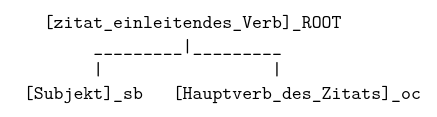
\includegraphics[width=0.6\linewidth]{./images/structure_citation.png}
	\end{center}
\caption{Subtree Repräsentation eines Syntaktischen Zitats}
\label{tree-general}
\end{figure}

Die möglichen Kategorien sind in der Tabelle \ref{legend-spacy-parsers} beschrieben. Diese Kategorien
widerspiegeln nicht konsequent Wortarten oder Begriffe aus der Satzlehre, wie sie im Deutschunterricht
gelehrt werden. Deshalb ist auch mit der Erklärung oft nicht klar, wofür sie stehen. Deren Auftreten
ist jedoch konsistent genug, sodass sie zur Erkennung der gewünschten Satzstrukturen genutzt werden
können.

\begin{table}[H]
    \centering
    \begin{tabular}{|l|r|}
        \hline
        \textbf{Spacy Parser Label} & \textbf{Spacy Erklärung} \\
        \hline
        \hline
        ROOT & root \\
        \hline
        da & dative \\
        \hline
        mnr & postnominal modifier \\
        \hline
        mo & modifier \\
        \hline
        nk & noun kernel element \\
        \hline
        oc & clausal object \\
        \hline
        punct & punctuation \\
        \hline
        sb & subject \\
        \hline
    \end{tabular}
    \caption{Legende zu den wichtigsten Spacy Parser Labels}
    \label{legend-spacy-parsers}
\end{table}

Die nachfolgenden Abbildungen \ref{tree-direct} und \ref{tree-indirect} sind konkrete Beispiele solcher
Trees. Der \gl{spacy-parser}  überrascht mit seiner Fähigkeit, Zitate in der direkten und
indirekten Rede gleich strukturieren zu können.

Die Abbildung \ref{tree-direct} repräsentiert den Satz
\enquote{Macron sagte zu Xi, »Die Aggression hat der Stabilität einen Schlag versetzt«.}
mit einem Zitat in der direkten Rede.

\begin{figure}[H]
	\begin{center}
        \centering
		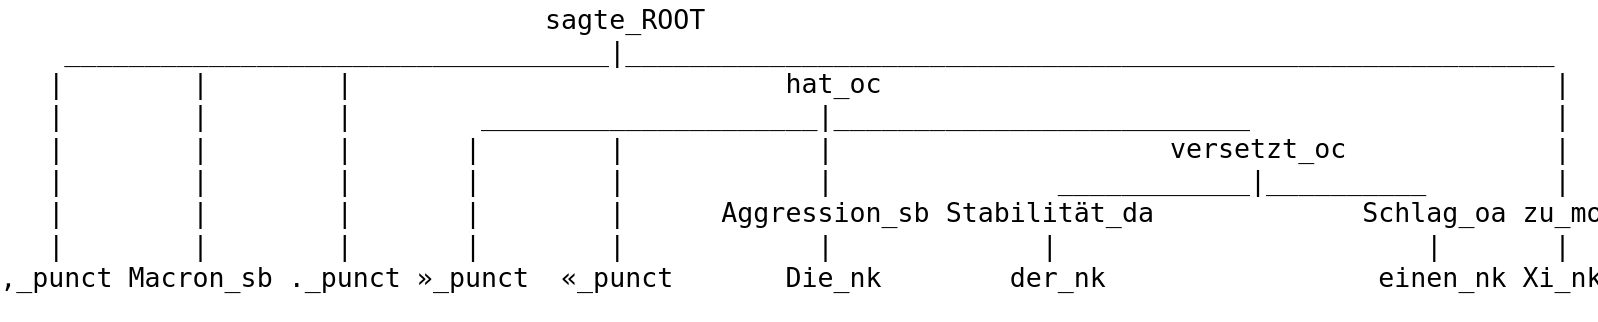
\includegraphics[width=\linewidth]{./images/macron-sagte-zu-xi-direkt.png}
	\end{center}
\caption{Parse Tree eines Satzes mit einem Syntaktischem Zitat in der direkten Rede}
\label{tree-direct}
\end{figure}

Die Abbildung \ref{tree-indirect} repräsentiert den Satz
\enquote{Macron sagte zu Xi dass die Aggression der Stabilität einen Schlag versetzt habe.}
mit einem Zitat in der indirekten Rede.

\begin{figure}[H]
	\begin{center}
        \centering
		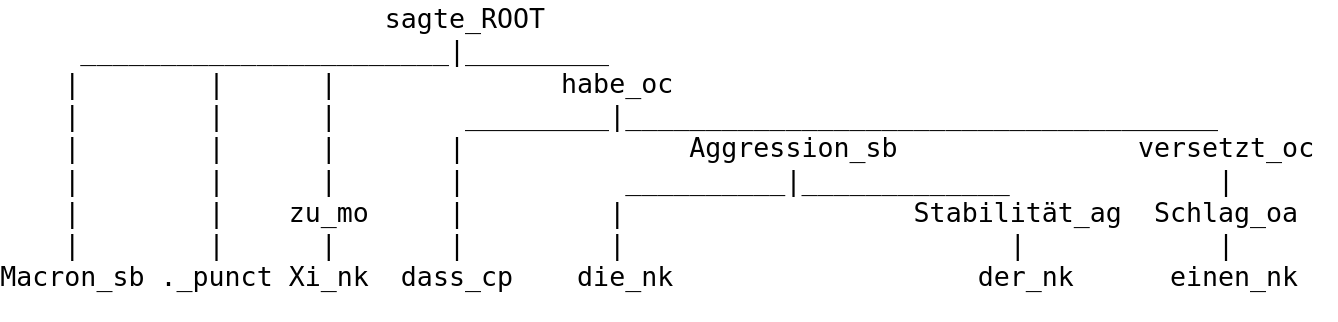
\includegraphics[width=\linewidth]{./images/macron-sagte-zu-xi-indirekt.png}
	\end{center}
\caption{Parse Tree eines Satzes mit einem Syntaktischem Zitat in der indirekten Rede.}
\label{tree-indirect}
\end{figure}

\subsection{Ablauf des Algorithmus}

Der nachfolgende Abschnitt soll konzeptuell und mit einigen Code-Beispielen erklären, wie der
Algorithmus vorgeht, um die Zitate in der oben beschriebenen Struktur zu Erkennen und zu extrahieren.

Hinweis: Im nachfolgenden Text werden die Terme \enquote{Node}, \enquote{Knoten} und \enquote{Token} als Synonyme verwendet.
Der Grund dafür ist, dass \enquote{Token} die Namensgebung von \gl{spacy}  ist und \enquote{Node} und \enquote{Knoten}
die passenden Begriffe dazu aus der Graphentheorie sind.

Der nachfolgende Code in Abbildung \ref{get-quotation-node} zeigt die Funktion, die das Programm verwendet,
um den \enquote{Hauptverb des Zitats} (vgl. Abbildung \ref{tree-general})
aus dem Parse Tree zu extrahieren. Gemeint ist damit derjenige Knoten, der als Kinder alle Wörter 
des Zitats enthält. Grundsätzlich muss die Funktion dabei unterscheiden, ob der vorliegende Satz 
in einer Zeitform mit Hilfsverb vorliegt (Perfekt, Plusquamperfekt oder Futur) oder in einer 
Zeitform ohne (Präsens oder Präteritum).

Die Funktion bedient sich einer weiteren Funktion \enquote{\_\_get\_nearest\_token\_by\_condition}
(vgl. Abbildung \ref{get-token-by-condition}), um in einer Breitensuche nach dem entsprechenden Node zu suchen.

\begin{figure}[H]
    \begin{lstlisting}[language=Python]
def __get_quote_node(root: Token) -> Token:
    result = []

    # Perfekt, Plusquamperfekt, Futur
    if root.lemma_ in __get_hilfsverben():
        condition = (
            lambda n: n.head.lemma_ in __get_quotation_verbs() and n.dep_ == "oc"
        )
        result = __get_flattened_list(
            [__get_nearest_tokens_by_condition(c, condition) for c in root.children]
        )

    # Präsens, Präteritum
    if root.lemma_ in __get_quotation_verbs():
        result = [x for x in root.children if x.dep_ == "oc"]

    if len(result) < 1:
        raise _NotFoundError()

    return result[0]
    \end{lstlisting}
    \caption{Function \_\_get\_quote\_node}
    \label{get-quotation-node}
\end{figure}

Die Funktion \enquote{\_\_get\_nearest\_token\_by\_condition} in der Abbildung \ref{get-token-by-condition} wird vom Algorithmus verwendet,
um die Knoten des Subjekts, des Zitat-einleitenden Verbes und des Zitats zu finden. Die Funktion
durchsucht den gegebenen Subtree mit der Strategie der Breitensuche, um den nächsten Knoten im Baum zu finden,
der eine vorgegebene Bedingung erfüllt. Die Bedingung ist dabei jeweils spezifisch für den gesuchten Knotentyp.

Das Resultat ist derjenige Knoten, der den kürzesten Pfad zum gegebenen Ursprungsknoten aufweist und die Bedingung erfüllt.

\begin{figure}[H]
    \begin{lstlisting}[language=Python]
# Breadth First Search
def __get_nearest_tokens_by_condition(
    node: Token, condition: Callable[[Token], bool]
) -> List[Token]:
    def get_nearest_by(
        node: Token, condition: Callable[[Token], bool], depth: int
    ) -> List[Tuple[Token, int]]:
        # check current node
        if condition(node):
            return [(node, depth)]

        # Recursion step (flatten result)
        return __get_flattened_list(
            [get_nearest_by(n, condition, depth + 1) for n in node.children]
        )

    results = get_nearest_by(node, condition, 0)
    if len(results) < 1:
        return []
    min_depth = min(results, key=lambda t: t[1])[1]

    return list(map(lambda t: t[0], filter(lambda t: t[1] == min_depth, results)))
    \end{lstlisting}
    \caption{Function \_\_get\_nearest\_token\_by\_condition}
    \label{get-token-by-condition}
\end{figure}

Da die identifizierte Struktur aus Abbildung \ref{tree-general} von \textsl{Syntaktischen Zitaten} nicht eindeutig ist, müssen die Zitat-Kandidaten
mithilfe einer Liste von \enquote{Zitat-einleitenden Verben} gefiltert werden, um False-Positives zu vermeiden.

Die nachfolgende Liste mit \enquote{Zitat einleitenden Verben} in Abbildung \ref{quotation-verbs} ist als Ressource im Projekt abgelegt.
Der Funktionsaufruf \textsl{\_\_get\_quotation\_verbs}  in Abbildung \ref{get-quotation-node} retourniert eine Python Liste mit diesen
Wörtern. Die Funktion \textsl{\_\_get\_quote\_node} verwendet diese Verben, um das \enquote{Zitat einleitende Verb} zu finden.

\begin{figure}[H]
    \begin{lstlisting}
ankündigen, argumentieren, aufrufen, begrüssen, behaupten, berichten, bestätigen, betonen, bezeichnen, bringen, dementieren, empfehlen, erklären, erwidern, erzählen, fassen, feststellen, fragen, kontern, kündigen, meinen, mitteilen, nennen, rechnen, rufen, sagen, schreiben, stellen, teilen, twittern, verraten, versichern, verweisen, werfen, zitieren, zusammenfassen
    \end{lstlisting}
    \caption{Quotation verbs}
    \label{quotation-verbs}
\end{figure}

Dieser Ansatz ist Fehleranfällig, da die Liste nicht abschliessend ist und Wörter fehlen, die Zitate einleiten können.
Die Verben müssen sehr spezifisch sein, weil ansonsten Satzstrukturen als Zitate erkannt werden, die gar keine sind.
Zitate, die mit unspezifischen Verben wie \enquote{sein} eingeleitet werden, können deshalb mit dieser Methode nicht erkannt werden.
Präzisionseinbussen sind wahrscheinliche Folgen (vgl. \ref{quality-assurance}).


